\section{Madelung treatment }
\begin{frame}
    \frametitle{Derivation from HF total energy}
\begin{align}
    \red{E_{\rm HF}}(N) &= \sum_{\mathbf k} \green{\frac{k^2}{2}}\, n_k + \green{E_x} - \frac{N\red{|v_M|}}{2} \label{eq:hf_energy_1} \\
    &= \sum_{\mathbf k} \left(\green{\frac{k^2}{2}} - \red{\frac{|v_M|}{2}}\right) n_k + \green{E_x} \label{eq:hf_energy_2}
\end{align}\pause
with $
    \green{\Sigma^x_k} = -\frac{1}{\Omega}\sum_{\mathbf{q}\neq0} v_q\, n_{\mathbf{k}+\mathbf{q}}$\pause and
$    \green{E_x} = -\frac{1}{2\Omega}\sum_{\mathbf{k}}\sum_{\mathbf{q}\neq0} v_q\, n_{\mathbf{k}} n_{\mathbf{k}+\mathbf{q}}
    = -\frac{1}{2\Omega}\sum_{\mathbf{k}\neq\mathbf{k}'} v_{\mathbf{k}-\mathbf{k}'}\, n_{\mathbf{k}} n_{\mathbf{k}'}
    = \frac{1}{2}\sum_{\mathbf{k}}\green{\Sigma^x_k}\, n_{\mathbf{k}}$.\pause Then,
\begin{align}
    \rm IP &\equiv \red{E_{\rm HF}}(N-1) - \red{E_{\rm HF}}(N), \quad     \rm EA \equiv \red{E_{\rm HF}}(N+1) - \red{E_{\rm HF}}(N)\\
    &= -\left(\green{\frac{i^2}{2}} + \green{\Sigma^x_i}\right) + \frac{\red{|v_M|}}{2}, \qquad =\left(\green{\frac{a^2}{2}} + \green{\Sigma^x_a}\right) - \frac{\red{|v_M|}}{2} 
    % &\equiv -\red{F^{\rm HF}_i},
\end{align} \pause
since $
    \green{E_x}(N-1)
    = \green{E_x}(N) - \green{\Sigma^x_i}$ and $
    \green{E_x}(N+1)
    = \green{E_x}(N) + \green{\Sigma^x_a}$.
\end{frame}
\begin{frame}
    \frametitle{Why this is the proper interpretation of your paper }
 I interpret what you write after equation 64 as saying that it makes no difference whether the Madelung constant gets lumped into the single-particle energies, as in Eq.~(\ref{eq:hf_energy_2}), or added afterwards as in Eq.~(\ref{eq:hf_energy_1}). \pause I interpret what you write after equation 66 as saying that 
\begin{align}
    E_g &\equiv EA + \frac{\red{|v_M|}}{2} + IP + \frac{\red{|v_M|}}{2}\\
    &= \left(\green{\frac{j^2}{2}} + \green{\Sigma^x_j} - \frac{\red{|v_M|}}{2}\right) + \left[-\left(\green{\frac{i^2}{2}} + \green{\Sigma^x_i}\right) + \frac{\red{|v_M|}}{2}\right]+ \red{|v_M|}\\
&= \green{\frac{j^2}{2}} + \green{\Sigma^x_j} - \green{\frac{i^2}{2}} - \green{\Sigma^x_i} + \red{|v_M|} \label{eq:band_gap_madelung}
\end{align}
\end{frame}
\begin{frame}
    \frametitle{Consistency with QCPBC convention}
Band gaps are consistent (equation~(\ref{eq:band_gap_madelung})). \pause Previously used shifted Ewald summation, where $v_q = \begin{cases} \frac{4\pi}{q^2}, & q\neq 0\\ -\Omega\red{v_M}, & q=0\end{cases}$\pause, so total energies were 
\begin{align}
    \red{E_{\rm HF}}(N) &= \sum_{\mathbf k} \green{\frac{k^2}{2}}\, n_k - \frac{1}{2}\sum_{\mathbf{k}} n_{\mathbf{k}}\left(\frac{1}{\Omega}\sum_{\mathbf{q}} v_q\, n_{\mathbf{k}+\mathbf{q}}\right) \\
    &= \sum_{\mathbf k} \green{\frac{k^2}{2}}\, n_k - \frac{1}{2}\sum_{\mathbf{k}} n_{\mathbf{k}}\left(\frac{1}{\Omega}\left[\sum_{\mathbf{q}\neq 0} v_q\, n_{\mathbf{k}+\mathbf{q}} + \Omega\red{|v_M|}\, n_{\mathbf{k}}\right]\right) \\
    &= \sum_{\mathbf k} \green{\frac{k^2}{2}}\, n_k + \frac{1}{2}\sum_{\mathbf{k}}\green{\Sigma^x_k}\, n_{\mathbf{k}} - \frac{\red{|v_M|}}{2}\sum_{\mathbf{k}} n_{\mathbf{k}}^2 \\
    &= \sum_{\mathbf k} \green{\frac{k^2}{2}}\, n_k + \green{E_x} - \frac{N\red{|v_M|}}{2}.
\end{align} \pause
Recall that HF energies came out to be $\varepsilon^{\rm HF}_k = \green{\frac{k^2}{2}} + \green{\Sigma^x_k} - \red{|v_M|}\, n_{\mathbf{k}}$.
\end{frame}
\begin{frame}
    \frametitle{How BW changes} Define $\green{E^{(0)}_{ij\to ab}} = \green{\varepsilon_a} + \green{\varepsilon_b} - \green{\varepsilon_i} - \green{\varepsilon_j}$. \pause 
Since $\operatorname{Tr}(\mathbf{W}^{O}) - \operatorname{Tr}(\mathbf{W}^{V})=E^{(2)}$, \pause
\textbf{Before} and \textbf{Now}, respectively:\begin{align}
\red{{E}^{(2)}} &= -\sum_{ijab}\frac{\green{\mathcal{K}_{ij}^{ab}}}{{\red{\tilde{E}_{ij\rightarrow ab}^{(0)}}}}\\
\red{\tilde{E}_{ij\rightarrow ab}^{(0)}}&= \green{E^{(0)}_{ij\to ab}}+2\red{|v_M|}\\
\Sigma^{(2)}_{pp}(\omega) &= \sum_{ija} \frac{\green{\mathcal{K}_{ij}^{ap}}}{\omega -\green{\epsilon^i} + \left( \green{\epsilon_a} - \green{\epsilon_j}\right) - 2\red{|v_M|}} + \sum_{iab} \frac{\green{\mathcal{K}_{ip}^{ab}}}{\omega-\green{\epsilon_a} - \left(\green{\epsilon_b} - \green{\epsilon_i}\right) + \red{|v_M|}} \end{align} \pause
\begin{align}
\green{E^{(2)}} &= -\sum_{ijab}\frac{\green{\mathcal{K}_{ij}^{ab}}}{{\green{E_{ij\rightarrow ab}^{(0)}}}}\\
\Sigma^{(2)}_{pp}(\omega)&= \sum_{ija} \frac{\green{\mathcal{K}_{ij}^{ap}}}{\omega-\green{\epsilon_i} + \left( \green{\epsilon_a} - \green{\epsilon_j}
\right)+ \frac{\red{|v_M|}}{2}} + \sum_{iab} \frac{\green{\mathcal{K}_{ip}^{ab}}}{\omega-\green{\epsilon_a} - \left(\green{\epsilon_b} - \green{\epsilon_i}\right)+ \frac{\red{|v_M|}}{2}}
\end{align}

\end{frame}
\begin{frame}
    \frametitle{Updated results: BW 4,0}
\begin{figure}
    \centering
    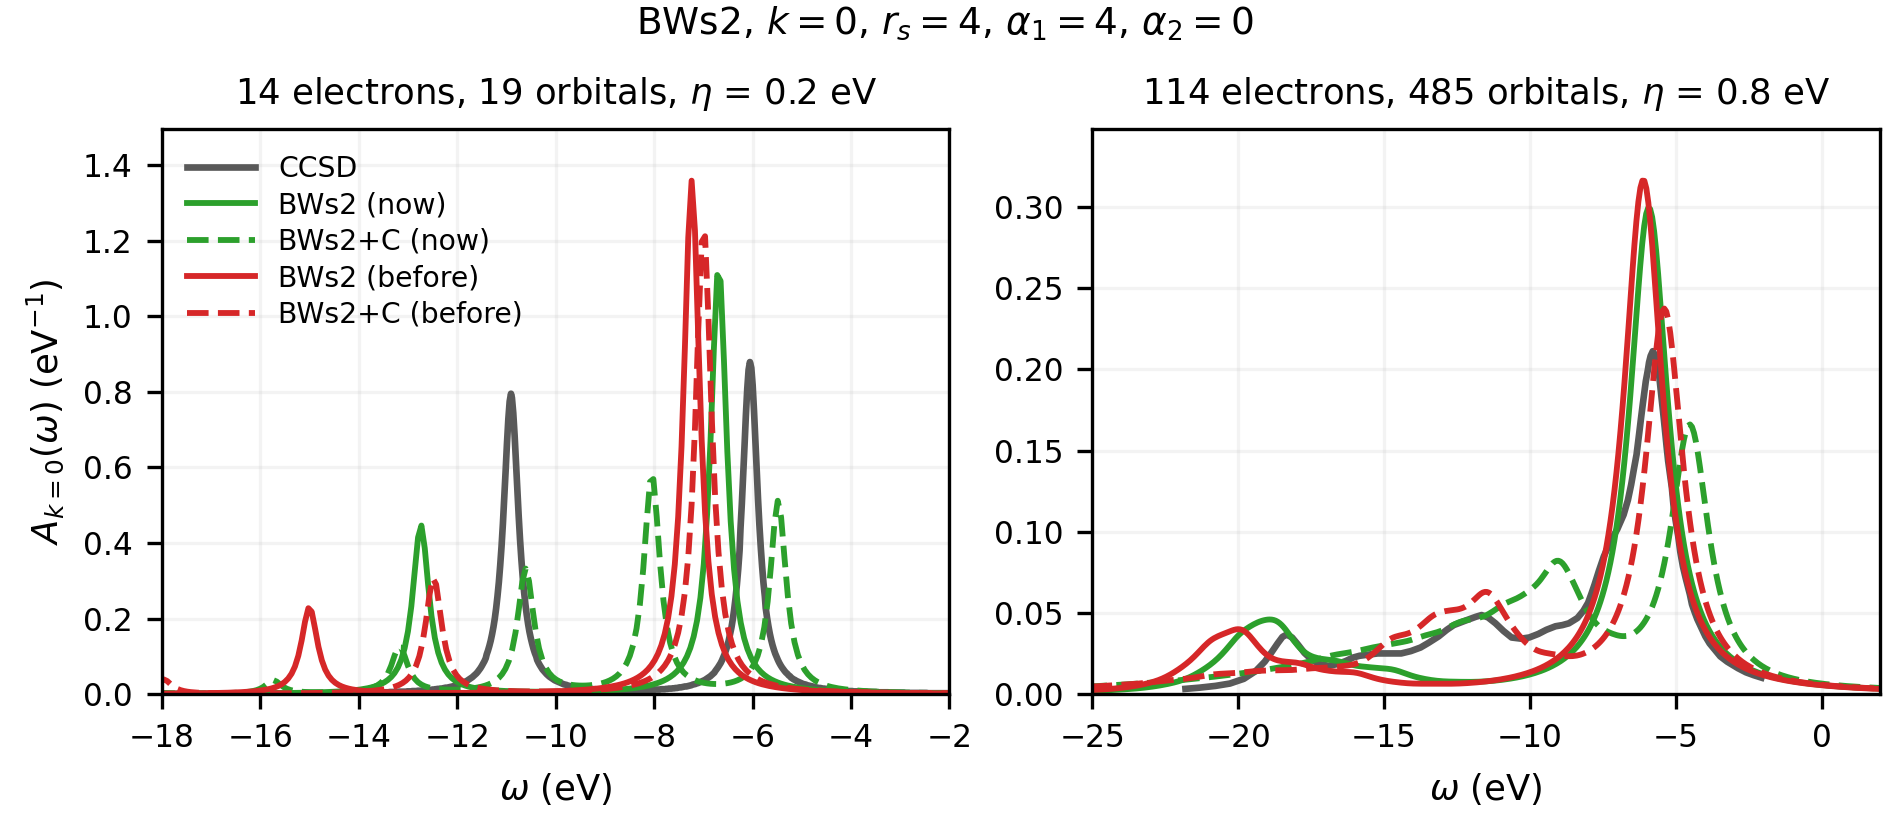
\includegraphics[width=\textwidth]{26/10/07/k0_twopanel_fig3_bws2_a40.png}
\end{figure}
\end{frame}
\begin{frame}
    \frametitle{Updated results: BW 2,2}
\begin{figure}
    \centering
    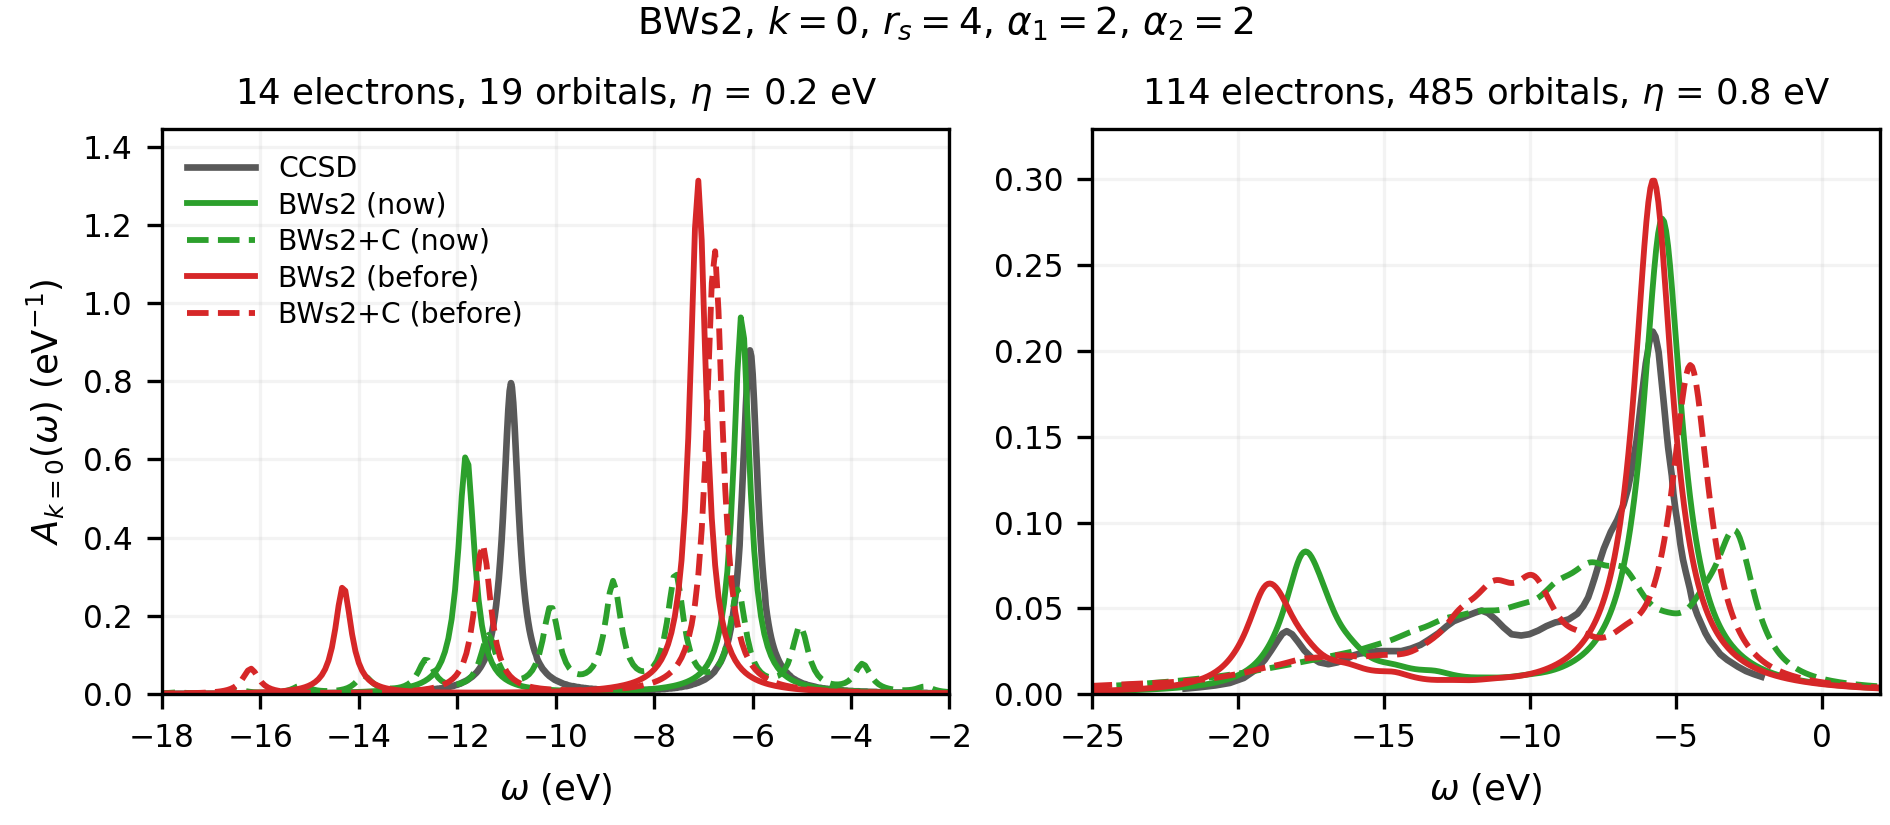
\includegraphics[width=\textwidth]{26/10/07/k0_twopanel_fig4_bws2_a22.png}
\end{figure}
\end{frame}
\begin{frame}
    \frametitle{How HF+GW changes}
1. Calculate the RPA polarizability   
\begin{align}
    &\left(\begin{array}{ll}
\mathrm{A} & \mathrm{~B} \\
\mathrm{~B} & \mathrm{~A}
\end{array}\right)\left(\begin{array}{ll}
\mathrm{X} & \mathrm{Y} \\
\mathrm{Y} & \mathrm{X}
\end{array}\right)=\left(\begin{array}{cc}
\mathrm{X} & -\mathrm{Y} \\
-\mathrm{Y} & \mathrm{X}
\end{array}\right)\left(\begin{array}{ll}
\Omega & 0 \\
0 & \Omega
\end{array}\right)\end{align} \pause
2. Form the correlation self-energy as
\begin{align}
\Sigma_{pp}^{c,G_0W_0}(\omega)&= \sum_{j \nu}\frac{W_{p j \nu} W_{p j \nu}}{\omega-\left(\epsilon_j-\Omega_\nu\right)-\mathrm{i} \eta} + \sum_{b \nu}\frac{W_{p b \nu} W_{p b \nu}}{\omega-\left(\epsilon_b+\Omega_\nu\right)+\mathrm{i} \eta},
\end{align}
where $W_{n p \nu}=\sqrt{2}\sum_{i a} V_{n p i a}(\mathbf{X}+\mathbf{Y})_{i a, \nu}$ with $V_{n p i a}=(n i|p a)$.
\end{frame}
\begin{frame}
    \frametitle{How HF+GW changes cont.}
\textbf{Before }:
\begin{align*}
    A_{ia,jb} &= \delta_{ij}\delta_{ab}\left(\green{\epsilon_a}-\green{\epsilon_i}+\red{|v_M|}\right)+\langle\Phi_i^a|\green{\hat V_{\rm res}}|\Phi_j^b\rangle\\
    &= \delta_{ij}\delta_{ab}\left(\green{\epsilon_a}-\green{\epsilon_i}\right)+\langle\Phi_i^a|\green{\hat V_{\rm res}}|\Phi_j^b\rangle\\
B_{ia,jb} &= \langle\Phi_i^a|\green{\hat V_{\rm res}}|\Phi_j^b\rangle \\
    \Sigma_{pp}^{c,G_0W_0}(\omega)&= \sum_{j \nu}\frac{\red{W_{p j \nu}} \red{W_{p j \nu}}}{\omega-\left(\green{\epsilon_j}-\red{|v_M|}-\red{\Omega_\nu}\right)+\mathrm{i} \eta} + \sum_{b \nu}\frac{\red{W_{p b \nu}} \red{W_{p b \nu}}}{\omega-\left(\green{\epsilon_b}+\red{\Omega_\nu}\right)+\mathrm{i} \eta}
\end{align*}
\pause 
\textbf{Now }: 
\begin{align}
    A_{ia,jb} &= \delta_{ij}\delta_{ab}\left(\green{\epsilon_a}-\red{\frac{|v_M|}{2}}-\green{\epsilon_i}+\red{\frac{|v_M|}{2}}\right)+\langle\Phi_i^a|\green{\hat V_{\rm res}}|\Phi_j^b\rangle\\
    &= \delta_{ij}\delta_{ab}\left(\green{\epsilon_a}-\green{\epsilon_i}\right)+\langle\Phi_i^a|\green{\hat V_{\rm res}}|\Phi_j^b\rangle\\
B_{ia,jb} &= \langle\Phi_i^a|\green{\hat V_{\rm res}}|\Phi_j^b\rangle \\
    \Sigma_{pp}^{c,G_0W_0}(\omega)&= \sum_{j \nu}\frac{\green{W_{p j \nu}} \green{W_{p j \nu}}}{\omega-\left(\green{\epsilon_j}+\red{\frac{v_M}{2}}-\green{\Omega_\nu}\right)+\mathrm{i} \eta} + \sum_{b \nu}\frac{\green{W_{p b \nu}} \green{W_{p b \nu}}}{\omega-\left(\green{\epsilon_b}+\red{\frac{v_M}{2}}+\green{\Omega_\nu}\right)+\mathrm{i} \eta}
\end{align}
\end{frame}
\begin{frame}
    \frametitle{Updated results: HF+GW}
\begin{figure}
    \centering
    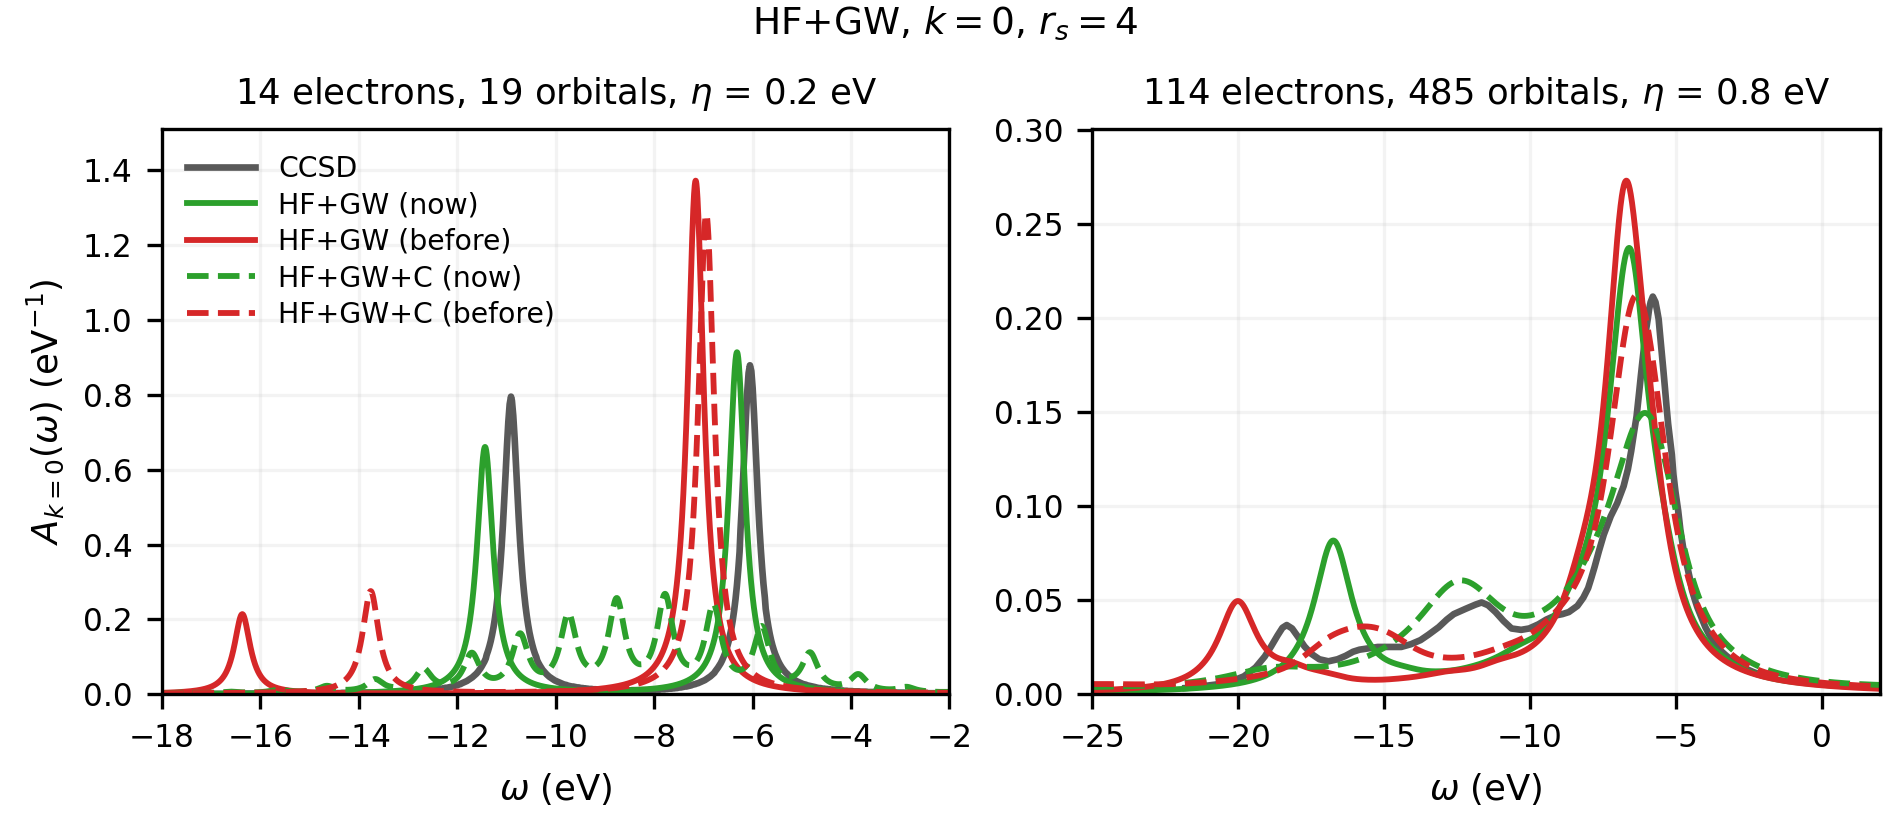
\includegraphics[width=\textwidth]{26/10/07/k0_twopanel_fig1a_hfgw_now_vs_before.png}
\end{figure}
\end{frame}
\begin{frame}
    \frametitle{Comparing updated HF+GW to LDA+GW}
\begin{figure}
    \centering
    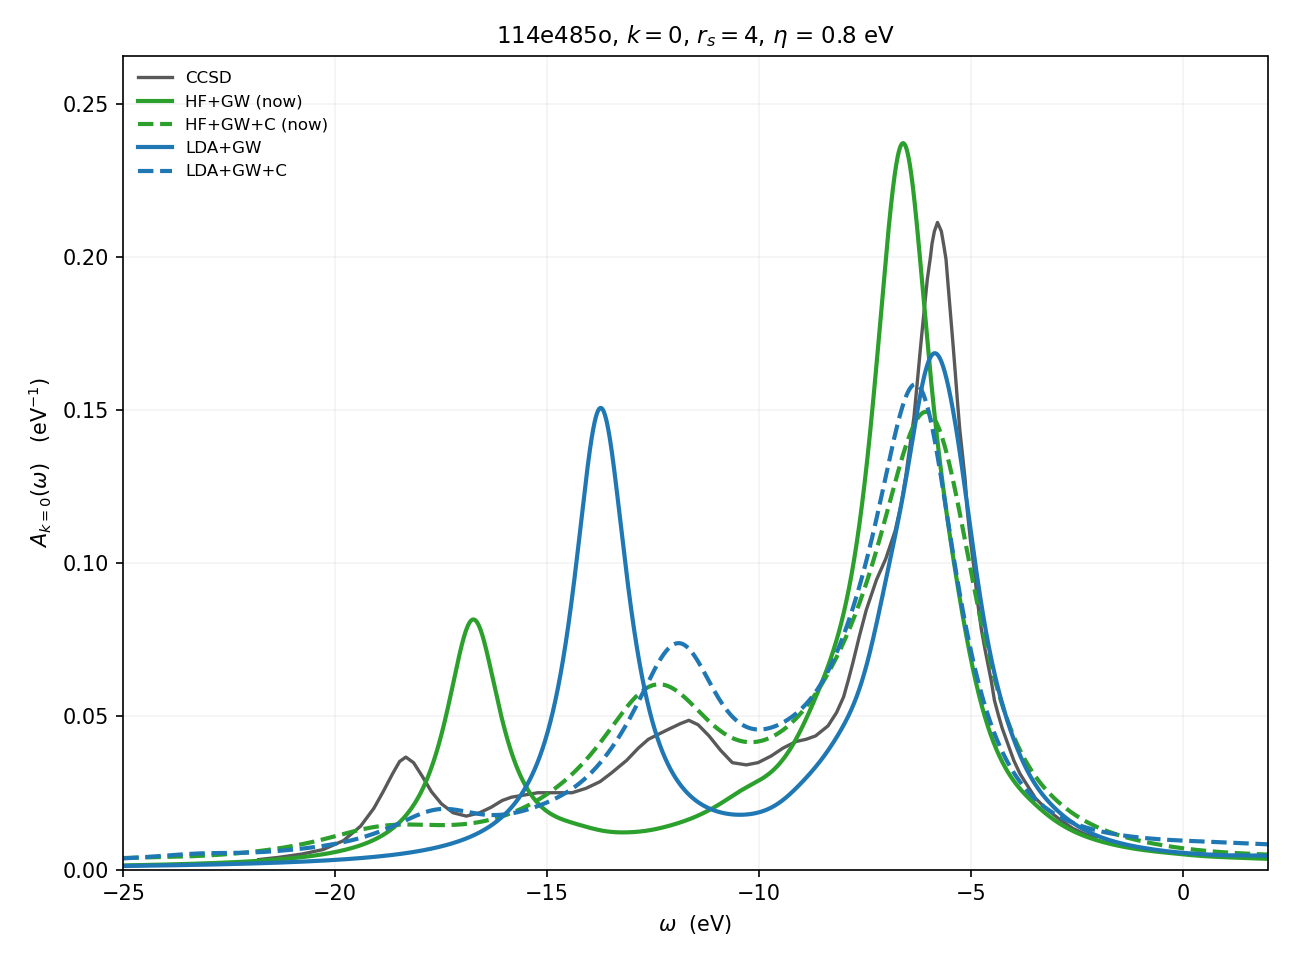
\includegraphics[width=0.9\textwidth]{26/10/07/k0_114e485o_fig1b_hfgw_now_vs_lda.png}
\end{figure}
\end{frame}
\begin{frame}
    \frametitle{Things to do now}
\begin{enumerate}
    \item Rerun Holm style SCCE(GW0) with Madelung correction. \pause
    \item Rerun CCSD with Madelung correction. \pause
\item Redo all TDL extrapolations with Madelung correction.
    \end{enumerate}
\end{frame}
\section{Derivation of the quasiboson Hamiltonian }
\begin{frame}
    \frametitle{The goal}
With $\epsilon_{\mathbf k}^{(0)}=\frac{k^2}{2}+\frac{v_M}{2}$ and $v_M=-2.837297 \times\left(\frac{3}{4 \pi}\right)^{1 / 3} N^{-1 / 3} r_s^{-1}$
\begin{align}
\hat H
&=
\sum_{\mathbf k}\epsilon_{\mathbf k}^{(0)}\hat a_{\mathbf k}^\dagger \hat a_{\mathbf k}
+
{\frac{1}{2\Omega}
\sum_{\mathbf q\neq\mathbf 0}v_q
\sum_{\mathbf k\mathbf k'}
a_{\mathbf{k}+\mathbf q}^\dagger
a_{\mathbf{k}'-\mathbf q}^\dagger
a_{\mathbf k'}
a_{\mathbf k}}\\
&=
E_{\rm HF}
+
{\sum_{\mathbf k}
\epsilon_{\mathbf k}^{\rm HF}
:
\hat a_{\mathbf k}^\dagger \hat a_{\mathbf k}
:}
+
\frac{1}{2\Omega}
\sum_{\mathbf q\neq\mathbf 0}v_q
\sum_{\mathbf k\mathbf k'}:
a_{\mathbf{k}+\mathbf q}^\dagger
a_{\mathbf{k}'-\mathbf q}^\dagger
a_{\mathbf k'}
a_{\mathbf k}:
\end{align}
where ${
\epsilon_{\mathbf k}^{\rm HF}
}
=
\frac{k^2}{2}
+
\frac{v_M}{2}
-
\frac{1}{\Omega}
\sum_{\mathbf q\neq\mathbf 0}
v_q n_{\mathbf{k}+\mathbf q}
$. \pause We want to get to 
\begin{equation}
    \hat H_{\rm eb}
    =
    -\sum_{\mathbf k\in\mathcal O}
    \epsilon_{\mathbf k}^{\rm HF}
    h_{\mathbf k}^{\dagger}h_{\mathbf k}
    +
    \sum_{\nu_{\mathbf q}}
    \omega_{\nu_{\mathbf q}}^{\rm pl}
    \hat\beta_{\nu_{\mathbf q}}^{\dagger}
    \hat\beta_{\nu_{\mathbf q}}
    +
    \sum_{\mathbf k\mathbf q}
    \sum_{\nu_{\mathbf q}}
    g_{\nu}^{\rm pl}(\mathbf k,\mathbf q)
    h_{\mathbf k+\mathbf q}^{\dagger}
    h_{\mathbf k}
    \left(
        \hat\beta_{\nu_{\mathbf q}}
        +
        \hat\beta_{\nu_{-\mathbf q}}^{\dagger}
    \right).
\end{equation}
\end{frame}
\begin{frame}
    \frametitle{Quadratic bosonic bath}
Define  $
    E_{i\mathbf q}^{\dagger}
    =
    a_{\mathbf{i}+\mathbf q}^{\dagger}a_{\mathbf i}$ and $
    E_{i\mathbf -q}
    =
    a_{\mathbf i}^{\dagger}a_{\mathbf{i}-\mathbf q}$ with $\hat\kappa[\mathbf z]
    =
    \sum_{i\mathbf q}
    \left[
        \kappa_{i\mathbf q}
        E_{i\mathbf q}^{\dagger}
        -
        \kappa_{i\mathbf q}^{*}
        E_{i\mathbf q}
    \right]$ using $
    \boldsymbol{\kappa}_{\mathbf q}
    =
    \begin{pmatrix}
        \kappa_{1\mathbf q}\\
        \kappa_{2\mathbf q}\\
        \vdots
    \end{pmatrix}
$ and $
    {
    \mathbf z_{\mathbf q}
    =
    \begin{pmatrix}
        \boldsymbol{\kappa}_{\mathbf q}\\
        \boldsymbol{\kappa}_{-\mathbf q}^{*}
    \end{pmatrix}
    }
$. \pause Given $    |\Phi(\mathbf z)\rangle
    =
    e^{\hat\kappa[\mathbf z]}
    |\Phi_0\rangle$, we have \begin{align}
    E(\mathbf z)
    &=
    \langle\Phi(\mathbf z)|
    \hat H
    |\Phi(\mathbf z)\rangle
    \\
    % &=
    % \langle\Phi_0|
    % e^{-\hat\kappa[\mathbf z]}
    % \hat H
    % e^{\hat\kappa[\mathbf z]}
    % |\Phi_0\rangle\\
    &=
    E_{\rm HF}
    +
    \langle\Phi_0|
    [\hat H,\hat\kappa[\mathbf z]]
    |\Phi_0\rangle
+
    \frac{1}{2}
    \langle\Phi_0|
    [[\hat H,\hat\kappa[\mathbf z]],\hat\kappa[\mathbf z]]
    |\Phi_0\rangle
    +
    \ldots \\ 
\implies     \nabla_{\mathbf z}E(\mathbf z)
    &=
    \begin{pmatrix}
        \dfrac{\partial E(\mathbf z)}
        {\partial\boldsymbol{\kappa}}\\
        \\
        \dfrac{\partial E(\mathbf z)}
        {\partial\boldsymbol{\kappa}^{*}}
    \end{pmatrix} \implies    \left.
    \nabla_{\mathbf z}E(\mathbf z)
    \right|_{\mathbf z=0}
    =
    0
    \label{eq:energy_expansion_kappa}
\end{align}
\end{frame}
\begin{frame}
    \frametitle{Quadratic bosonic bath cont.}
\begin{align}
    \mathcal H_{\rm HF}
    =
    \left.
    \frac{\partial^2 E(\mathbf z)}
    {\partial
    \begin{pmatrix}
        \boldsymbol{\kappa}^{*}\\
        \boldsymbol{\kappa}
    \end{pmatrix}
    \partial
    \begin{pmatrix}
        \boldsymbol{\kappa}&
        \boldsymbol{\kappa}^{*}
    \end{pmatrix}}
    \right|_{\mathbf z=0}
    &={
    \begin{pmatrix}
        A & B\\
        B^{*} & A^{*}
    \end{pmatrix}.
    }
\end{align} \pause
Thus, the second-order correction to the HF energy is
\begin{align}
E^{(2)}(\mathbf \kappa, \mathbf \kappa^{*})
    &=
    \frac{1}{2}
    \begin{pmatrix}
        \boldsymbol{\kappa}_{\mathbf q}^{*} &
        \boldsymbol{\kappa}_{-\mathbf q}
    \end{pmatrix}
    \begin{pmatrix}
        A & B\\
        B^{*} & A^{*}
    \end{pmatrix}
    \begin{pmatrix}
        \boldsymbol{\kappa}_{\mathbf q}\\
        \boldsymbol{\kappa}_{-\mathbf q}^{*}
    \end{pmatrix}
\end{align}\pause
Quantizing the space and then applying Bogoliubov transformation gives 
\begin{align}
    \hat{H}^{(2)}&= \frac{1}{2}
    \begin{pmatrix}
        \hat{\bm{b}}_{\mathbf q}^{\dagger} &
        \hat{\bm{b}}_{-\mathbf q}
    \end{pmatrix}
    \begin{pmatrix}
        A & B\\
        B^{*} & A^{*}
    \end{pmatrix}
    \begin{pmatrix}
        \hat{\bm{b}}_{\mathbf q}\\
        \hat{\bm{b}}_{-\mathbf q}^{\dagger}
    \end{pmatrix}\\
    &=
    \hat{\bm{\beta}}_{\mathbf q}^{\dagger} \boldsymbol{\Omega}_{\mathbf q} \hat{\bm{\beta}}_{\mathbf q}
    +
    \frac{1}{2}\operatorname{Tr}(\boldsymbol{\Omega}_{\mathbf q}-A)+\frac{1}{2}\operatorname{Tr}(A)\\
&= \sum_{\nu_{\mathbf q}} \omega_{\nu_{\mathbf q}} \hat{\beta}_{\nu_{\mathbf q}}^{\dagger} \hat{\beta}_{\nu_{\mathbf q}} + E_{\rm RPA} + \frac{1}{2}\operatorname{Tr}(A)
\end{align}
\end{frame}
\begin{frame}
    \frametitle{Pure fermionic and coupling terms}
Start with 
\begin{equation}
    \hat H_{\rm h}(\boldsymbol{\kappa})
    =
    \sum_{\mathbf k,\mathbf k'\in\mathcal O}
    h^{\rm h}_{\mathbf k'\mathbf k}(\boldsymbol{\kappa})
    h_{\mathbf k'}^\dagger h_{\mathbf k}.
    \label{eq:hole_hamiltonian_kappa}
\end{equation} \pause Expand to first order about the
Hartree--Fock reference
\begin{align}
    h^{\rm h}_{\mathbf k'\mathbf k}(\boldsymbol{\kappa})
    &=
    h^{\rm h}_{\mathbf k'\mathbf k}(0)+
    \sum_{i\mathbf q}
    \left.
    \frac{\partial
    h^{\rm h}_{\mathbf k'\mathbf k}}
    {\partial\kappa_{i\mathbf q}}
    \right|_{0}
    \kappa_{i\mathbf q}+
    \sum_{i\mathbf q}
    \left.
    \frac{\partial
    h^{\rm h}_{\mathbf k'\mathbf k}}
    {\partial\kappa_{i\mathbf q}^{*}}
    \right|_{0}
    \kappa_{i\mathbf q}^{*}
    +
    \mathcal O(\kappa^2),
    \label{eq:hole_hamiltonian_expansion}
\end{align} 
\pause
\begin{align}
    \left.
    \frac{\partial
    h^{\rm h}_{\mathbf k+\mathbf q,\mathbf k}}
    {\partial\kappa_{i\mathbf q}}
    \right|_0
    &=
    -
    \left.
    \frac{\partial
    F_{\mathbf k,\mathbf k+\mathbf q}}
    {\partial\kappa_{i\mathbf q}}
    \right|_0
    \\
    &=
    -
    \sum_{\mathbf l}
    \frac{\partial
    F_{\mathbf k,\mathbf k+\mathbf q}}
    {\partial P_{\mathbf l + \mathbf q,\mathbf l}}
    \left.
    \frac{\partial
    P_{\mathbf l + \mathbf q,\mathbf l}}
    {\partial\kappa_{i\mathbf q}}
    \right|_0 \\
&= 
    -
\frac{v(\mathbf q)}{\Omega} \sum_{\mathbf l}
    \delta_{\mathbf l,\mathbf i}
\end{align}
\end{frame}
\begin{frame}
    \frametitle{Pure fermionic and coupling terms cont.}
So up to linear order in $\boldsymbol{\kappa}$
\begin{align}
    \hat H_{\rm h}(\boldsymbol{\kappa})
    &\overset{\text{direct}}{=} -
    \sum_{\mathbf k\in\mathcal O}
    \epsilon_{\mathbf k}^{\rm HF}
    h_{\mathbf k}^{\dagger}h_{\mathbf k}
-
    \sum_{\mathbf k\mathbf q}
    \sum_i
    \frac{v(\mathbf q)}{\Omega}
    h_{\mathbf k+\mathbf q}^{\dagger}h_{\mathbf k}
    \left(
        \kappa_{i\mathbf q}
        +
        \kappa_{i,-\mathbf q}^{*}
    \right)
    \label{eq:hole_hamiltonian_linear_kappa}
\end{align} \pause
Quantizing again and then applying the Bogoliubov transformation gives
\begin{align}
    \hat H_{\rm h-pl}
    &=
    \sum_{\mathbf k\mathbf q}
    \sum_{\nu_{\mathbf q}}
    g_{\nu}^{\rm pl}(\mathbf k,\mathbf q)
    h_{\mathbf k+\mathbf q}^{\dagger}
    h_{\mathbf k}
    \left(
        \hat\beta_{\nu_{\mathbf q}}
        +
        \hat\beta_{\nu_{-\mathbf q}}^{\dagger}
    \right),
    \label{eq:hole_plasmon_coupling}
\end{align} \pause
with
\begin{equation}
    {
    g_{\nu}^{\rm pl}(\mathbf k,\mathbf q)
    =
    -\frac{v(\mathbf q)}{\Omega}
    \sum_{\mathbf i}
    \left[
        X_{i\nu}(\mathbf q)
        +
        Y_{i\nu}(\mathbf q)
    \right].
    }
    \label{eq:screened_hole_plasmon_coupling}
\end{equation}\pause
So overall (omitting constant terms)
\begin{equation}
    \hat H_{\rm eb}
    =
    -\sum_{\mathbf k\in\mathcal O}
    \epsilon_{\mathbf k}^{\rm HF}
    h_{\mathbf k}^{\dagger}h_{\mathbf k}
    +
    \sum_{\nu_{\mathbf q}}
    \omega_{\nu_{\mathbf q}}^{\rm pl}
    \hat\beta_{\nu_{\mathbf q}}^{\dagger}
    \hat\beta_{\nu_{\mathbf q}}
    +
    \sum_{\mathbf k\mathbf q}
    \sum_{\nu_{\mathbf q}}
    g_{\nu}^{\rm pl}(\mathbf k,\mathbf q)
    h_{\mathbf k+\mathbf q}^{\dagger}
    h_{\mathbf k}
    \left(
        \hat\beta_{\nu_{\mathbf q}}
        +
        \hat\beta_{\nu_{-\mathbf q}}^{\dagger}
    \right).
\end{equation}


\end{frame}
\begin{frame}
    \frametitle{Results}
\begin{figure}
    \centering
    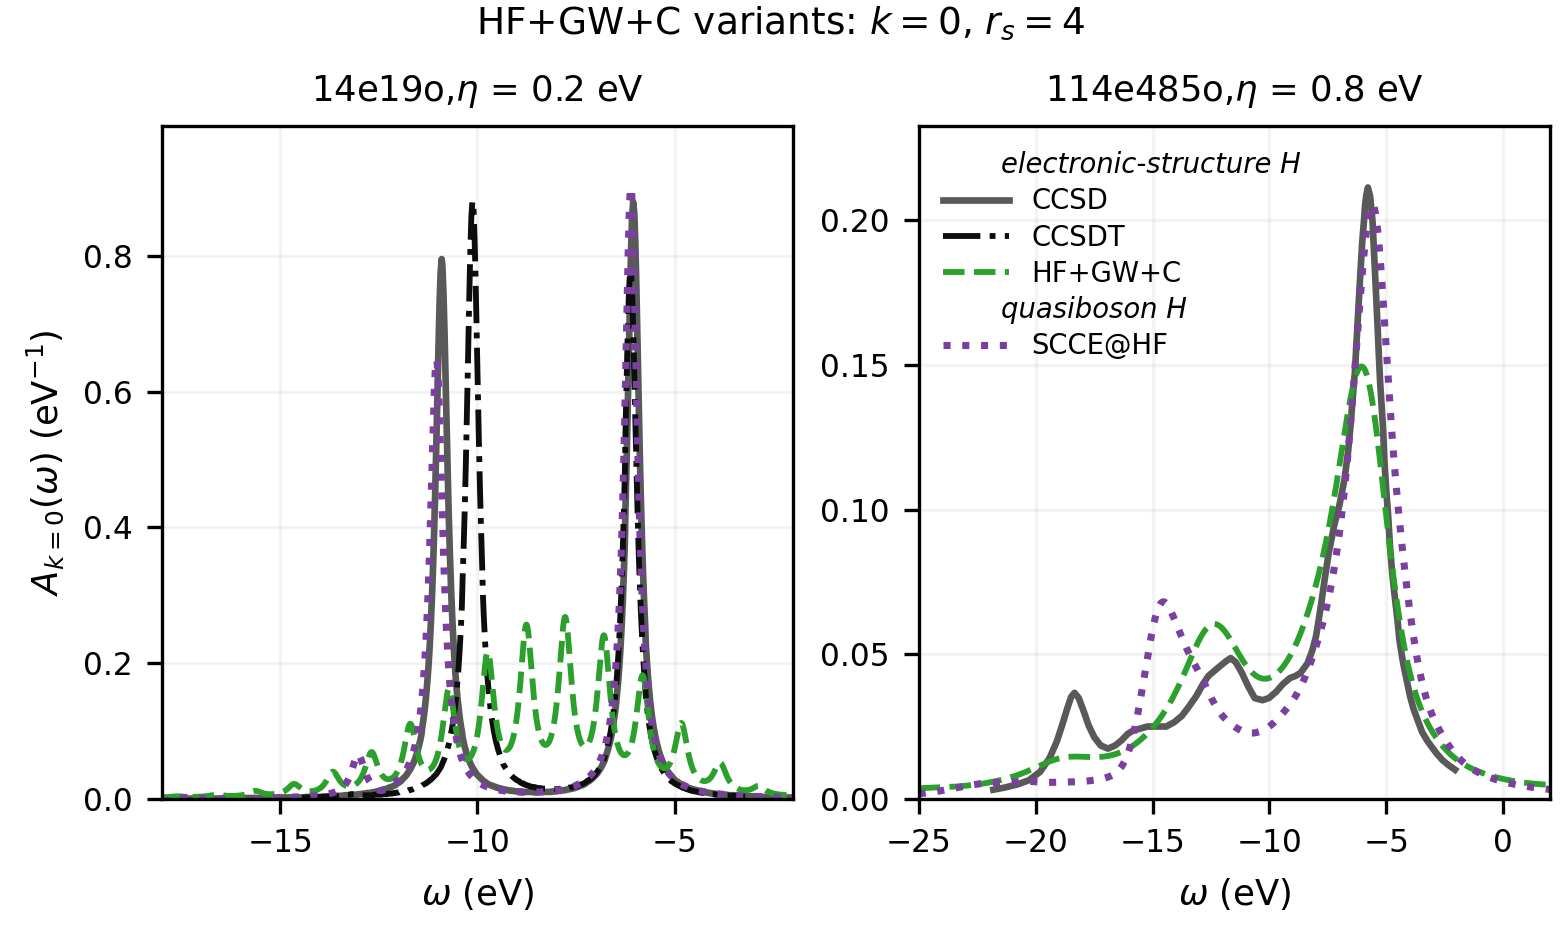
\includegraphics[width=\textwidth]{26/10/07/k0_twopanel_fig5_es_vs_qb.png}
\end{figure}
\end{frame}
\begin{frame}
    \frametitle{Results}
\begin{figure}
    \centering
    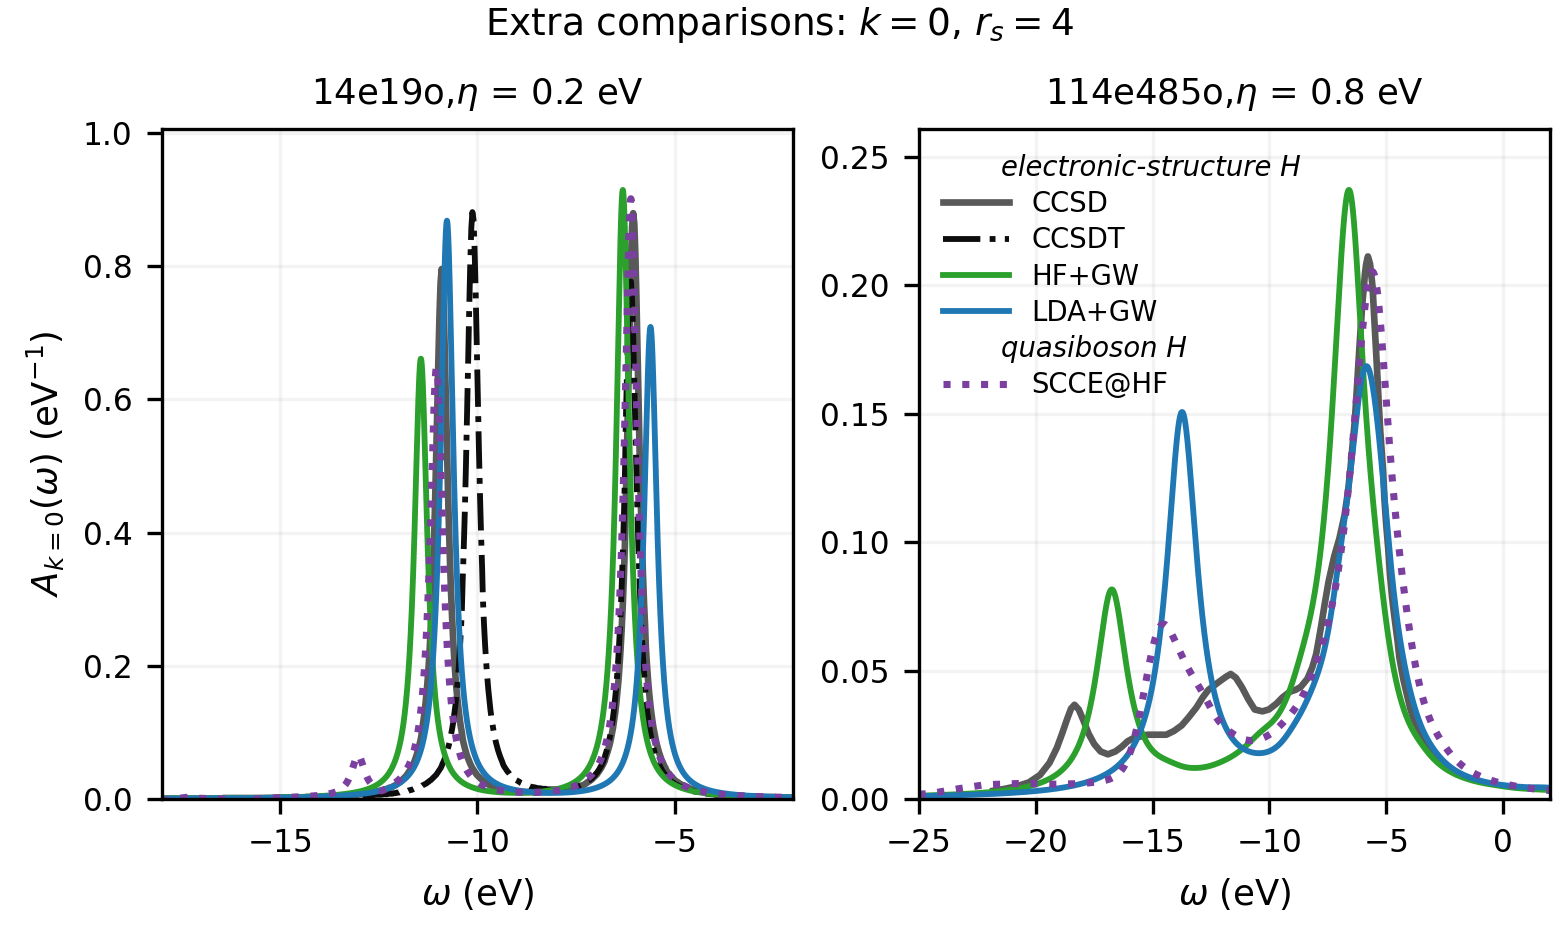
\includegraphics[width=\textwidth]{26/10/07/k0_twopanel_fig6_gw_frames_vs_scce.png}
\end{figure}
\end{frame}